\documentclass[11pt]{article}
\usepackage[utf8]{inputenc}
\usepackage[T1]{fontenc}
\usepackage{lmodern}
\usepackage{amsmath,amssymb}
\usepackage{graphicx}
\usepackage{booktabs}
\usepackage{float}
\usepackage[a4paper,margin=2.4cm]{geometry}
\usepackage{caption}
\usepackage{subcaption}
\usepackage{enumitem}
\usepackage[hidelinks]{hyperref}

\renewcommand{\figurename}{Figura}
\renewcommand{\tablename}{Tabela}
\renewcommand{\refname}{Referências}
\renewcommand{\contentsname}{Sumário}
\renewcommand{\abstractname}{Resumo}
\captionsetup{font=small}

\title{\textbf{Otimização Bioobjetivo da Alocação de Máquinas Virtuais em\\
Computação em Nuvem com Colônia de Formigas (VMPACS)}\\[4pt]
\large Seminário de Algoritmos Bioinspirados}
\author{Lucas Rivetti \qquad Ian Nunes}
\date{Junho de 2026}

\usepackage{fancyhdr}
\pagestyle{fancy}\fancyhf{}\fancyfoot[R]{\thepage}\renewcommand{\headrulewidth}{0pt}
\fancypagestyle{plain}{\fancyhf{}\fancyfoot[R]{\thepage}\renewcommand{\headrulewidth}{0pt}}
\begin{document}
\maketitle

\begin{abstract}
\noindent Este trabalho estuda e aplica um algoritmo bioinspirado
\emph{multiobjetivo} --- o \textbf{VMPACS} (\emph{Virtual Machine Placement Ant
Colony System}), proposto por Gao et al. (2013) --- ao problema biobjetivo de
\textbf{alocação de máquinas virtuais (VMs)} em \emph{data centers} de nuvem. O
objetivo é encontrar um conjunto de soluções não-dominadas (fronteira de Pareto)
que minimizem \emph{simultaneamente} o \textbf{consumo de energia} e o
\textbf{desperdício de recursos}. Implementamos o VMPACS fielmente ao artigo e o
comparamos com o \textbf{NSGA-II}, um algoritmo genético multiobjetivo clássico.
Os experimentos seguem a metodologia do artigo (instâncias com diferentes
correlações entre CPU e memória) e a qualidade das soluções é avaliada por meio
de \textbf{quatro métricas} de desempenho (Hipervolume, IGD, ONVG e
\emph{Spacing}), além dos indicadores práticos de energia, desperdício e número
de servidores. Os resultados mostram que ambos os algoritmos obtêm
empacotamentos compactos e de boa qualidade; o NSGA-II converge, em geral, para
soluções de menor energia e desperdício, enquanto o VMPACS tende a fornecer
fronteiras ligeiramente mais diversificadas.
\end{abstract}

\tableofcontents
\vspace{6pt}\hrule\vspace{6pt}

% =========================================================================
\section{Descrição do problema}
% =========================================================================
A virtualização é a tecnologia central da computação em nuvem: ela permite que
vários ambientes isolados (as \emph{máquinas virtuais}, VMs) compartilhem um
mesmo servidor físico. A \textbf{alocação de máquinas virtuais}
(\emph{VM placement}) é o processo de decidir \emph{em qual servidor físico cada
VM será executada}. Essa decisão é crítica porque governa diretamente o
\textbf{custo operacional} de um \emph{data center}, dominado pelo consumo de
energia, e o \textbf{aproveitamento dos recursos} (CPU e memória).

Do ponto de vista do provedor, deseja-se \emph{consolidar} as VMs no menor número
possível de servidores (desligando os ociosos para poupar energia), mas sem
sobrecarregar nem desbalancear os servidores ativos. O problema é uma variante do
\emph{empacotamento vetorial} (\emph{vector bin packing}), que é NP-difícil:
para $n$ VMs e $m$ servidores existem $m^{n}$ alocações possíveis, tornando a
enumeração completa inviável. Por isso recorremos a \textbf{meta-heurísticas
bioinspiradas}.

\paragraph{Por que é um problema multiobjetivo.} Reduzir o número de servidores
diminui a energia, mas pode forçar empacotamentos desbalanceados (por exemplo, um
servidor com a CPU cheia e a memória quase vazia), elevando o desperdício.
Tratamos, portanto, energia e desperdício como \emph{dois objetivos
conflitantes} e buscamos o conjunto de soluções de melhor compromisso (a
fronteira de Pareto), em vez de uma única solução.

% =========================================================================
\section{Objetivos de otimização}
% =========================================================================
Cada servidor é caracterizado por duas dimensões de recurso: \textbf{CPU} e
\textbf{memória}. Sejam $U^{p}_{j}$ e $U^{m}_{j}$ as utilizações (frações)
de CPU e memória do servidor $j$.

\begin{itemize}[leftmargin=1.4em]
  \item \textbf{Objetivo 1 --- Consumo de energia.} Medições mostram que a
  potência de um servidor cresce linearmente com a utilização de CPU. Servidores
  ociosos são desligados. A potência do servidor $j$ é
  \begin{equation}
    P_{j} = (P^{busy}_{j}-P^{idle}_{j})\,U^{p}_{j} + P^{idle}_{j},
    \qquad \text{se } U^{p}_{j}>0,\ \text{senão } 0,
    \label{eq:pot}
  \end{equation}
  com $P^{idle}=162$\,W e $P^{busy}=215$\,W (valores do artigo). Minimizar
  $\sum_j P_j$ equivale, na prática, a \emph{minimizar o número de servidores
  ligados}.

  \item \textbf{Objetivo 2 --- Desperdício de recursos.} Para aproveitar bem
  \emph{as duas} dimensões e mantê-las equilibradas, o desperdício do servidor
  $j$ é
  \begin{equation}
    W_{j} = \frac{\lvert L^{p}_{j}-L^{m}_{j}\rvert + \varepsilon}
                 {U^{p}_{j}+U^{m}_{j}},
    \label{eq:desp}
  \end{equation}
  onde $L^{p}_{j}$ e $L^{m}_{j}$ são os recursos de CPU e memória
  \emph{restantes} no servidor e $\varepsilon=10^{-4}$. O termo
  $\lvert L^{p}_{j}-L^{m}_{j}\rvert$ penaliza o \emph{desbalanceamento} entre as
  sobras de CPU e memória.
\end{itemize}

% =========================================================================
\section{Formulação matemática}
% =========================================================================
Sejam $n$ VMs ($i\in I$) a serem alocadas em $m$ servidores ($j\in J$). Cada VM
$i$ tem demanda de CPU $R^{p}_{i}$ e de memória $R^{m}_{i}$; cada servidor $j$ tem
limites (\emph{thresholds}) $T^{p}_{j}$ e $T^{m}_{j}$. Definimos as variáveis
binárias:
\[
  x_{ij}=\begin{cases}1,&\text{se a VM }i\text{ é alocada no servidor }j\\0,&\text{caso contrário}\end{cases}
  \qquad
  y_{j}=\begin{cases}1,&\text{se o servidor }j\text{ está em uso}\\0,&\text{caso contrário.}\end{cases}
\]
O problema biobjetivo é:
\begin{align}
  \min \quad & f_{1}=\sum_{j=1}^{m} y_{j}\!\left[(P^{busy}_{j}-P^{idle}_{j})\sum_{i=1}^{n} x_{ij}R^{p}_{i} + P^{idle}_{j}\right] \label{eq:f1}\\[2pt]
  \min \quad & f_{2}=\sum_{j=1}^{m} y_{j}\,
     \frac{\left\lvert\bigl(T^{p}_{j}-\sum_{i} x_{ij}R^{p}_{i}\bigr)-\bigl(T^{m}_{j}-\sum_{i} x_{ij}R^{m}_{i}\bigr)\right\rvert+\varepsilon}
          {\sum_{i} x_{ij}R^{p}_{i}+\sum_{i} x_{ij}R^{m}_{i}} \label{eq:f2}
\end{align}
sujeito a:
\begin{align}
  \sum_{j=1}^{m} x_{ij} &= 1, & &\forall i\in I, \label{eq:c1}\\
  \sum_{i=1}^{n} R^{p}_{i}\,x_{ij} &\le T^{p}_{j}\,y_{j}, & &\forall j\in J, \label{eq:c2}\\
  \sum_{i=1}^{n} R^{m}_{i}\,x_{ij} &\le T^{m}_{j}\,y_{j}, & &\forall j\in J, \label{eq:c3}\\
  x_{ij},\,y_{j} &\in \{0,1\}, & &\forall i\in I,\ \forall j\in J. \label{eq:c4}
\end{align}
A restrição~\eqref{eq:c1} garante que cada VM seja alocada em exatamente um
servidor; \eqref{eq:c2} e~\eqref{eq:c3} impõem os limites de CPU e memória de cada
servidor; \eqref{eq:c4} define o domínio das variáveis. Usamos
$T^{p}_{j}=T^{m}_{j}=0{,}9$ (90\%) para evitar a degradação de desempenho que
ocorre próximo de 100\% de utilização.

% =========================================================================
\section{Algoritmos utilizados}
% =========================================================================
\subsection{VMPACS --- Sistema de Colônia de Formigas}
O VMPACS é uma adaptação do \emph{Ant Colony System} (ACS) ao problema. A
metáfora biológica é a de formigas que, ao buscar alimento, depositam
\textbf{feromônio} nos caminhos percorridos; caminhos bons acumulam mais
feromônio e atraem mais formigas. Aqui, cada ``formiga'' constrói uma alocação
completa e os bons \emph{movimentos} (alocar a VM $i$ no servidor $j$) recebem
mais feromônio.

\paragraph{Feromônio e heurística.} O feromônio $\tau_{ij}$ indica a
conveniência de colocar a VM $i$ no $j$-ésimo servidor aberto. É inicializado com
$\tau_{0}=1/\!\left[n\,(P'(S_{0})+W(S_{0}))\right]$, onde $S_{0}$ é a solução da
heurística \emph{First-Fit Decreasing} (FFD). A informação heurística combina a
contribuição parcial de cada movimento aos dois objetivos:
\begin{equation}
  \eta_{ij}=\eta_{ij}^{(1)}+\eta_{ij}^{(2)},\quad
  \eta_{ij}^{(1)}=\frac{1}{\varepsilon+\sum_{v=1}^{j} P_{v}/P^{\max}_{v}},\quad
  \eta_{ij}^{(2)}=\frac{1}{\varepsilon+\sum_{v=1}^{j} W_{v}}.
  \label{eq:eta}
\end{equation}

\paragraph{Construção da solução (regra pseudoaleatória proporcional).} Para
escolher a próxima VM a empacotar no servidor atual, sorteia-se $q\sim U[0,1]$:
\begin{equation}
  i=\begin{cases}
     \displaystyle\arg\max_{u\in\Omega}\ \{\alpha\,\tau_{uj}+(1-\alpha)\,\eta_{uj}\}, & q\le q_{0}\ \text{(intensificação)}\\[6pt]
     s\ \text{sorteado por } p_{uj}=\dfrac{\alpha\,\tau_{uj}+(1-\alpha)\,\eta_{uj}}{\sum_{w\in\Omega}\alpha\,\tau_{wj}+(1-\alpha)\,\eta_{wj}}, & q> q_{0}\ \text{(exploração),}
    \end{cases}
  \label{eq:regra}
\end{equation}
onde $\Omega$ é o conjunto de VMs que ainda cabem no servidor atual e $\alpha$
pondera feromônio \emph{vs.} heurística.

\paragraph{Atualização do feromônio.} Há dois passos. A atualização
\emph{local}, aplicada a cada movimento construído, evita estagnação:
\begin{equation}
  \tau_{ij}\leftarrow(1-\rho_{l})\,\tau_{ij}+\rho_{l}\,\tau_{0}.
  \label{eq:local}
\end{equation}
A atualização \emph{global}, aplicada apenas às soluções da fronteira de Pareto
(arquivo externo) ao fim de cada iteração, reforça os bons movimentos:
\begin{equation}
  \tau_{ij}\leftarrow(1-\rho_{g})\,\tau_{ij}+\frac{\rho_{g}\,\lambda}{P'(S)+W(S)},
  \qquad \lambda=\frac{N_{A}}{t-N_{Is}+1},
  \label{eq:global}
\end{equation}
em que $t$ é a iteração atual e $N_{Is}$ a iteração em que a solução $S$ entrou no
arquivo. O Algoritmo~\ref{alg:vmpacs} resume o procedimento.

\begin{figure}[H]
\centering
\fbox{\parbox{0.94\textwidth}{\small
\textbf{Algoritmo 1: VMPACS} \\[2pt]
\textbf{Entrada:} VMs e servidores com demandas e limites; parâmetros
$\alpha,\rho_l,\rho_g,q_0,N_A,M$.\\
\textbf{Saída:} arquivo de Pareto $P$.\\[3pt]
1\quad Inicializa $P\leftarrow\varnothing$ e todo $\tau_{ij}\leftarrow\tau_0$\\
2\quad \textbf{para} $t=1$ \textbf{até} $M$ \textbf{faça}\\
3\quad\quad \textbf{para} cada formiga $1..N_A$ \textbf{faça}\\
4\quad\quad\quad abre um servidor; enquanto houver VMs que cabem: escolhe uma por~\eqref{eq:regra}\\
5\quad\quad\quad e aplica a atualização local~\eqref{eq:local}; repete abrindo novos servidores\\
6\quad\quad\quad avalia $(f_1,f_2)$ e atualiza o arquivo de não-dominadas $P$\\
7\quad\quad \textbf{para} cada solução $S\in P$: aplica a atualização global~\eqref{eq:global}\\
8\quad \textbf{retorna} $P$
}}
\caption{Pseudocódigo do VMPACS.}
\label{alg:vmpacs}
\end{figure}

\subsection{NSGA-II --- Algoritmo Genético Multiobjetivo (comparação)}
Para comparação, usamos o \textbf{NSGA-II} (Deb et al., 2002), o algoritmo
genético multiobjetivo mais difundido --- assim como o artigo original compara o
VMPACS com um algoritmo genético (MGGA). Seus dois mecanismos centrais são:
(i)~a \emph{ordenação por não-dominância}, que classifica a população em frentes
de Pareto sucessivas; e (ii)~a \emph{distância de multidão} (\emph{crowding}),
que preserva a diversidade ao longo da fronteira. Cada indivíduo é uma
\textbf{permutação} das VMs, decodificada pela heurística \emph{first-fit}
(garantindo soluções sempre válidas); os operadores são o \emph{Order Crossover}
(OX) e a mutação por troca (\emph{swap}). A seleção usa torneio binário baseado em
(frente, \emph{crowding}) e elitismo $(\mu+\lambda)$.

% =========================================================================
\section{Metodologia experimental}
% =========================================================================
\paragraph{Instâncias.} Geramos instâncias com $n=100$ VMs e $m=100$ servidores
homogêneos, reproduzindo o gerador correlacionado do artigo: a demanda de CPU é
sorteada em $[0,2\bar{R}_p)$ e a de memória em $[0,\bar{R}_m)$, com
$\bar{R}_p=\bar{R}_m=0{,}25$; um parâmetro $P\in[0,1]$ controla a
\textbf{correlação} entre CPU e memória. Usamos cinco níveis,
$P\in\{0;0{,}25;0{,}5;0{,}75;1{,}0\}$, correspondentes a coeficientes de
correlação aproximados de $-0{,}75$ (negativa forte) a $+0{,}75$ (positiva forte).

\paragraph{Parâmetros dos algoritmos.} VMPACS (valores do artigo): $N_A=10$
formigas, $M=100$ iterações, $\alpha=0{,}45$, $\rho_l=\rho_g=0{,}35$, $q_0=0{,}8$.
NSGA-II: população $50$, $20$ gerações, taxa de mutação $0{,}4$. Os orçamentos
foram \emph{equiparados} em $\approx\!1000$ avaliações de solução por execução,
para uma comparação justa.

\paragraph{Métricas de desempenho.} Avaliamos a qualidade das fronteiras com
quatro métricas consagradas:
\begin{itemize}[leftmargin=1.4em,itemsep=1pt]
  \item \textbf{Hipervolume (HV)} --- área do espaço de objetivos dominada pela
  fronteira em relação a um ponto de referência; \emph{maior é melhor} (mede
  convergência \emph{e} diversidade).
  \item \textbf{IGD} (\emph{Inverted Generational Distance}) --- distância média
  de uma fronteira de referência até a fronteira obtida; \emph{menor é melhor}.
  \item \textbf{ONVG} --- número de soluções não-dominadas encontradas;
  cardinalidade da fronteira.
  \item \textbf{\emph{Spacing} (SP)} --- uniformidade do espaçamento entre as
  soluções; \emph{menor é melhor}.
\end{itemize}
Para HV e IGD, os objetivos são normalizados em $[0,1]$ por nível de correlação, e
a fronteira de referência do IGD é a união das soluções não-dominadas de ambos os
algoritmos. Cada configuração é executada $R=10$ vezes de forma independente;
reportamos média\,$\pm$\,desvio-padrão. Para visualizar o trade-off real, calculamos ainda uma fronteira de Pareto de \emph{referência} (varredura do número de servidores com busca local, módulo \texttt{referencia.py}).

% =========================================================================
\section{Resultados}
% =========================================================================
A Figura~\ref{fig:barras} compara os \textbf{indicadores práticos} (energia,
desperdício e número de servidores) entre os algoritmos, nos cinco níveis de
correlação. A Figura~\ref{fig:mo} apresenta as \textbf{métricas multiobjetivo}
(Hipervolume e IGD) e exemplos de \textbf{fronteiras de Pareto} no espaço de
objetivos. As Tabelas~\ref{tab:t2}, \ref{tab:t1} e~\ref{tab:t3} trazem os valores
numéricos.

\begin{figure}[H]
\centering
\begin{subfigure}{0.48\textwidth}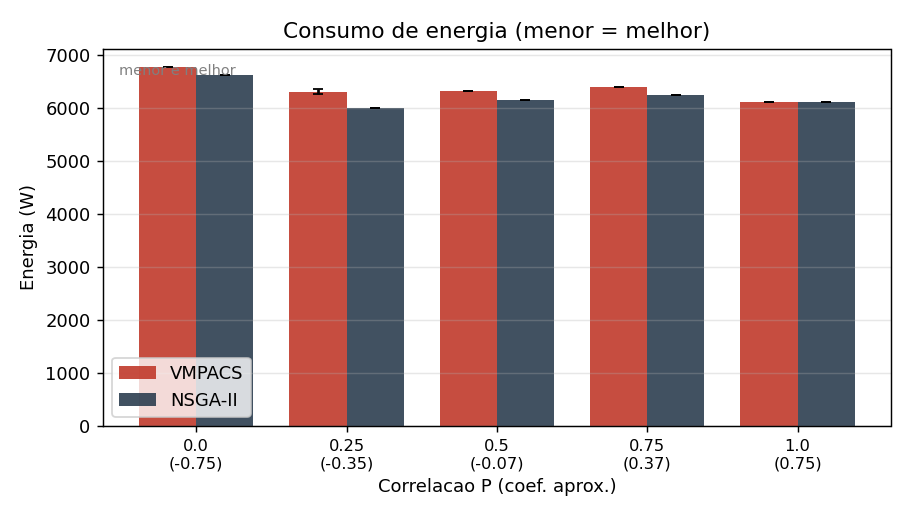
\includegraphics[width=\linewidth]{figuras/energia_barras.png}\end{subfigure}\hfill
\begin{subfigure}{0.48\textwidth}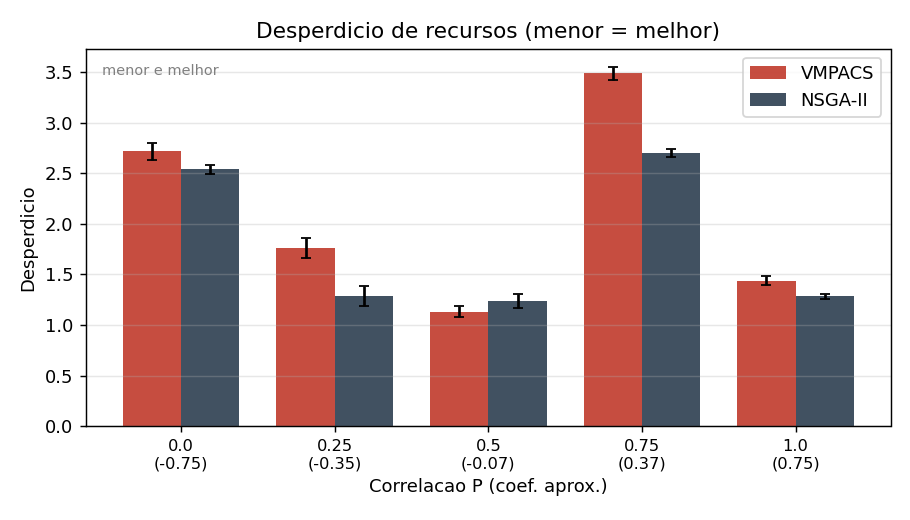
\includegraphics[width=\linewidth]{figuras/desperdicio_barras.png}\end{subfigure}
\\[4pt]
\begin{subfigure}{0.48\textwidth}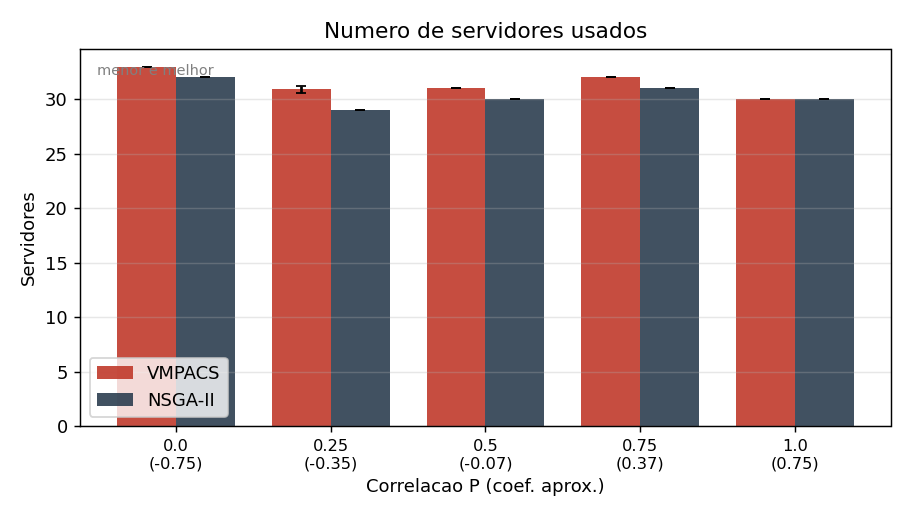
\includegraphics[width=\linewidth]{figuras/servidores_barras.png}\end{subfigure}
\caption{Indicadores práticos por nível de correlação $P$ (coeficiente aproximado
entre parênteses): energia, desperdício e número de servidores. Em todos,
\emph{menor é melhor}.}
\label{fig:barras}
\end{figure}

\begin{figure}[H]
\centering
\begin{subfigure}{0.48\textwidth}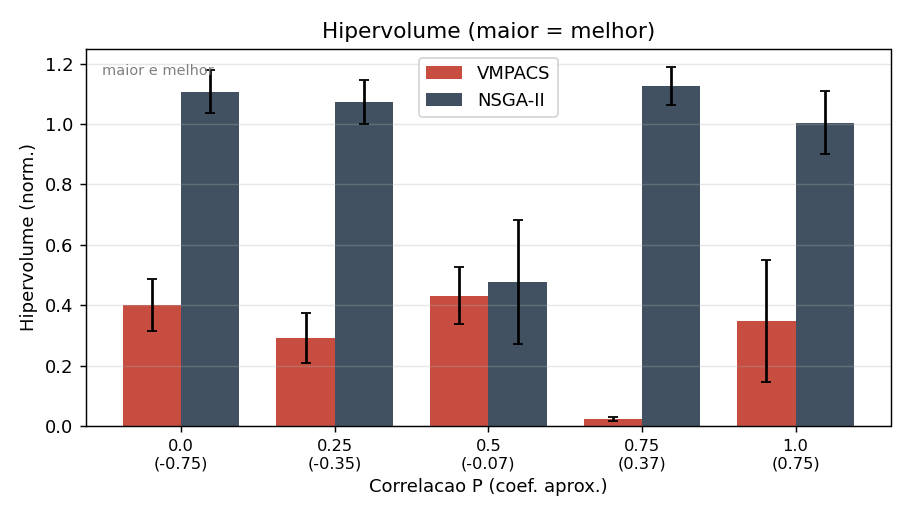
\includegraphics[width=\linewidth]{figuras/hipervolume_barras.png}\end{subfigure}\hfill
\begin{subfigure}{0.48\textwidth}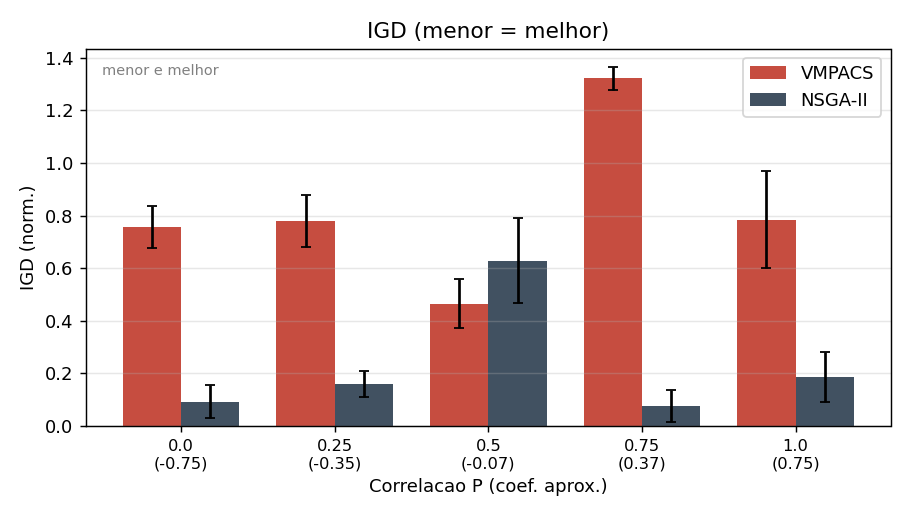
\includegraphics[width=\linewidth]{figuras/igd_barras.png}\end{subfigure}
\\[4pt]
\begin{subfigure}{0.99\textwidth}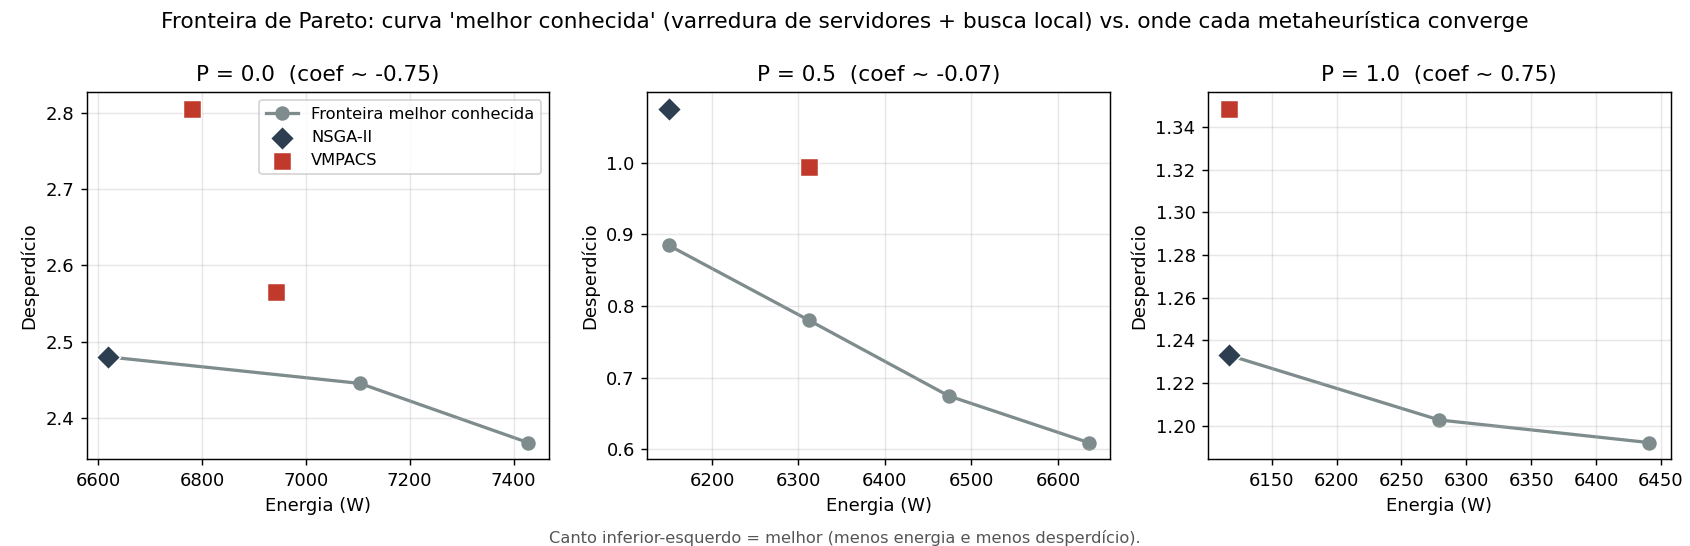
\includegraphics[width=\linewidth]{figuras/fronteiras_pareto.png}\end{subfigure}
\caption{Métricas multiobjetivo (Hipervolume --- maior é melhor; IGD --- menor é
melhor) e fronteiras de Pareto. Na fronteira, a curva cinza é a \emph{melhor conhecida}
(varredura do número de servidores + busca local) e os marcadores mostram onde cada
metaheurística converge. O canto inferior-esquerdo corresponde às melhores soluções.}
\label{fig:mo}
\end{figure}

\begin{table}[H]
\centering\small
\caption{Energia, desperdício e número de servidores (média\,$\pm$\,desvio).}
\label{tab:t2}
\begin{tabular}{cclccc}
\toprule
$P$ & coef. & Algoritmo & Energia (W) & Desperdício & Servidores \\
\midrule
0{,}00 & $-0{,}75$ & VMPACS  & $6780{,}2\pm0{,}0$ & $2{,}720\pm0{,}084$ & $33{,}0$ \\
                         &           & NSGA-II & $\mathbf{6618{,}2}\pm0{,}0$ & $\mathbf{2{,}540}\pm0{,}041$ & $\mathbf{32{,}0}$ \\
\addlinespace
0{,}25 & $-0{,}35$ & VMPACS  & $6302{,}4\pm48{,}6$ & $1{,}761\pm0{,}097$ & $30{,}9$ \\
       &           & NSGA-II & $\mathbf{5994{,}6}\pm0{,}0$ & $\mathbf{1{,}286}\pm0{,}098$ & $\mathbf{29{,}0}$ \\
\addlinespace
0{,}50 & $-0{,}07$ & VMPACS  & $6311{,}8\pm0{,}0$ & $\mathbf{1{,}131}\pm0{,}054$ & $31{,}0$ \\
       &           & NSGA-II & $\mathbf{6149{,}8}\pm0{,}0$ & $1{,}234\pm0{,}069$ & $\mathbf{30{,}0}$ \\
\addlinespace
0{,}75 & $+0{,}37$ & VMPACS  & $6402{,}6\pm0{,}0$ & $3{,}492\pm0{,}066$ & $32{,}0$ \\
       &           & NSGA-II & $\mathbf{6240{,}6}\pm0{,}0$ & $\mathbf{2{,}700}\pm0{,}042$ & $\mathbf{31{,}0}$ \\
\addlinespace
1{,}00 & $+0{,}75$ & VMPACS  & $6117{,}2\pm0{,}0$ & $1{,}440\pm0{,}048$ & $30{,}0$ \\
       &           & NSGA-II & $6117{,}2\pm0{,}0$ & $\mathbf{1{,}282}\pm0{,}025$ & $30{,}0$ \\
\bottomrule
\end{tabular}
\end{table}

\begin{table}[H]
\centering\small
\begin{minipage}{0.48\textwidth}\centering
\caption{ONVG e \emph{Spacing} (média).}
\label{tab:t1}
\begin{tabular}{clcc}
\toprule
$P$ & Algoritmo & ONVG & SP \\
\midrule
0{,}00 & VMPACS  & $2{,}1$ & $0{,}018$ \\
       & NSGA-II & $1{,}1$ & $0{,}000$ \\
0{,}25 & VMPACS  & $2{,}9$ & $0{,}097$ \\
       & NSGA-II & $1{,}4$ & $0{,}000$ \\
0{,}50 & VMPACS  & $1{,}2$ & $0{,}000$ \\
       & NSGA-II & $1{,}2$ & $0{,}000$ \\
0{,}75 & VMPACS  & $1{,}0$ & $0{,}000$ \\
       & NSGA-II & $1{,}3$ & $0{,}000$ \\
1{,}00 & VMPACS  & $1{,}0$ & $0{,}000$ \\
       & NSGA-II & $1{,}0$ & $0{,}000$ \\
\bottomrule
\end{tabular}
\end{minipage}\hfill
\begin{minipage}{0.48\textwidth}\centering
\caption{Hipervolume e IGD (média).}
\label{tab:t3}
\begin{tabular}{clcc}
\toprule
$P$ & Algoritmo & HV & IGD \\
\midrule
0{,}00 & VMPACS  & $0{,}400$ & $0{,}758$ \\
       & NSGA-II & $\mathbf{1{,}108}$ & $\mathbf{0{,}093}$ \\
0{,}25 & VMPACS  & $0{,}293$ & $0{,}779$ \\
       & NSGA-II & $\mathbf{1{,}072}$ & $\mathbf{0{,}160}$ \\
0{,}50 & VMPACS  & $0{,}432$ & $\mathbf{0{,}466}$ \\
       & NSGA-II & $\mathbf{0{,}478}$ & $0{,}629$ \\
0{,}75 & VMPACS  & $0{,}024$ & $1{,}322$ \\
       & NSGA-II & $\mathbf{1{,}127}$ & $\mathbf{0{,}077}$ \\
1{,}00 & VMPACS  & $0{,}347$ & $0{,}785$ \\
       & NSGA-II & $\mathbf{1{,}004}$ & $\mathbf{0{,}187}$ \\
\bottomrule
\end{tabular}
\end{minipage}
\end{table}

% =========================================================================
\section{Análise dos resultados}
% =========================================================================
\paragraph{Convergência (energia, desperdício, HV e IGD).} Pela
Tabela~\ref{tab:t2}, o NSGA-II obtém \emph{menor consumo de energia} em quatro dos
cinco níveis de correlação (empatando em $P=1{,}0$) e usa, em média, um servidor a
menos. O \emph{desperdício} também é menor para o NSGA-II em quatro casos, com
exceção de $P=0{,}5$, onde o VMPACS é ligeiramente melhor ($1{,}131$ contra
$1{,}234$). Essa vantagem do NSGA-II se reflete nas métricas multiobjetivo
(Tabela~\ref{tab:t3}): seu \textbf{Hipervolume} é maior e seu \textbf{IGD} é menor
na maioria dos cenários --- novamente, $P=0{,}5$ é a exceção, em que o VMPACS
alcança o melhor IGD ($0{,}466$). Ou seja, o NSGA-II em geral aproxima-se mais do
canto ideal do espaço de objetivos.

\paragraph{Diversidade (ONVG e \emph{Spacing}).} A Tabela~\ref{tab:t1} mostra um
ponto a favor do VMPACS: para correlações \emph{negativas} ($P=0$ e $P=0{,}25$)
ele encontra \emph{mais} soluções não-dominadas (ONVG de $2{,}1$ e $2{,}9$ contra
$\approx\!1$ do NSGA-II), oferecendo ao decisor um leque maior de compromissos. O
\emph{Spacing} é praticamente nulo porque as fronteiras têm poucos pontos.

\paragraph{Fronteiras compactas: objetivos quase alinhados.} O achado mais
importante da análise é que, para estas instâncias, as fronteiras de Pareto são
\emph{compactas} (poucos pontos --- ver Figura~\ref{fig:mo}). A razão é estrutural:
empacotar as VMs de forma \emph{justa e equilibrada} tende a reduzir
\emph{simultaneamente} a energia (poucos servidores) e o desperdício (servidores
balanceados). Os dois objetivos, embora formalmente distintos, ficam
\emph{fortemente correlacionados de forma positiva} nas instâncias aleatórias,
de modo que o conflito --- e portanto o número de soluções de compromisso --- é
pequeno. Esse comportamento é coerente com o artigo, cujos principais resultados
também são comparações \emph{agregadas} de energia e desperdício. A Figura~\ref{fig:mo} (parte inferior) torna isso explícito: a curva \emph{melhor conhecida} mostra que o trade-off existe, porém é raso. As metaheurísticas, com orçamento de $\approx$1000 avaliações, convergem para o joelho de menor energia; o NSGA-II encosta na fronteira, enquanto o VMPACS --- por minimizar servidores sem refinar tanto o balanceamento --- fica um pouco acima dela, o que aponta um \emph{refinamento por busca local (versão memética)} como melhoria direta.

\paragraph{Por que a fronteira não é uma curva suave?} Porque a energia vale exatamente $f_1=\text{const}+P^{idle}\cdot k$, com $k$ inteiro igual ao número de servidores: ela só assume valores \emph{discretos}, de $162$\,W em $162$\,W. A fronteira é, portanto, um conjunto de \emph{pontos} (um por número de servidores) e não uma curva contínua. Além disso, o desperdício \emph{satura}: com 2 a 3 servidores a mais que o mínimo os servidores já ficam bem equilibrados, e acrescentar mais apenas gasta energia --- por isso poucos pontos são não-dominados. A Figura~\ref{fig:forma} mostra a curva completa do compromisso: ela \emph{é} decrescente e convexa (o formato esperado de uma fronteira de Pareto), porém discreta e rasa, consequência direta de os dois objetivos serem quase alinhados.

\begin{figure}[H]\centering
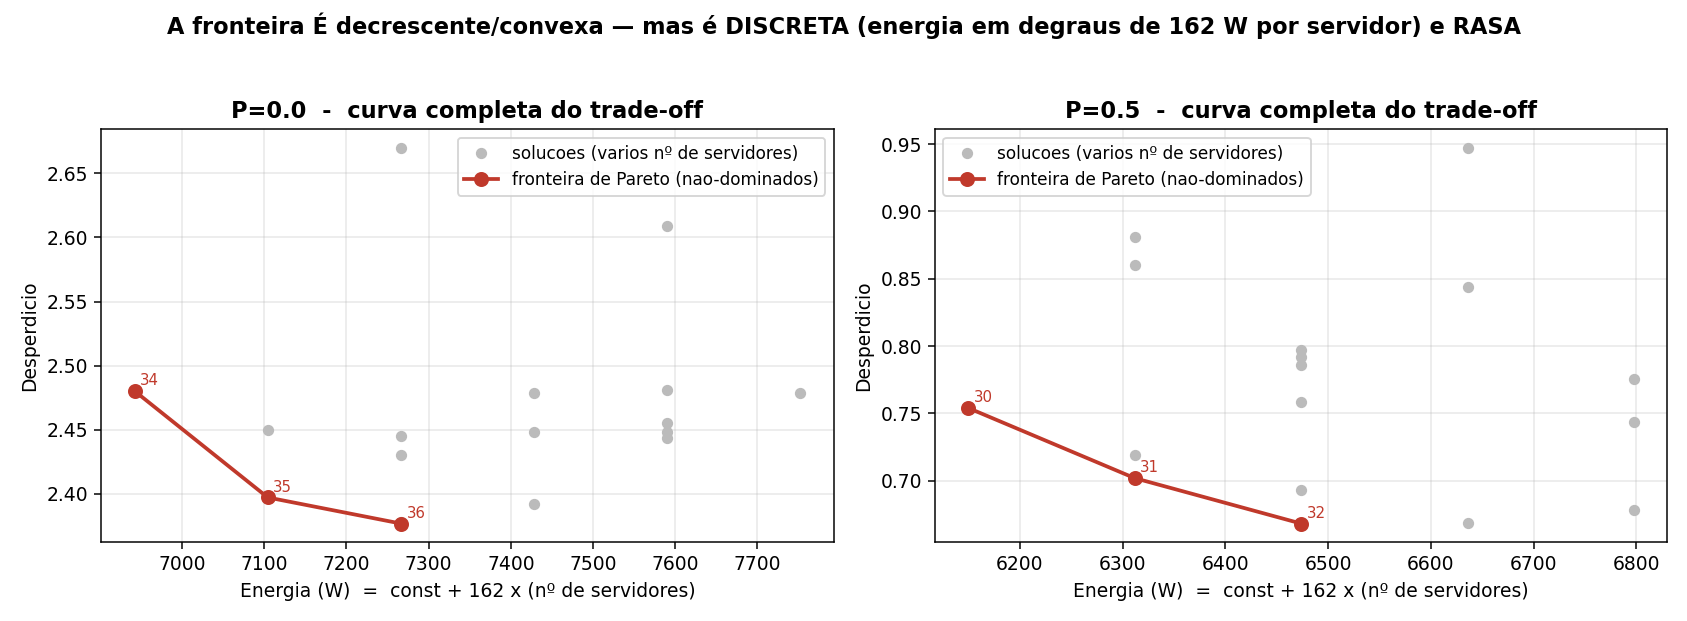
\includegraphics[width=0.96\textwidth]{figuras/forma_pareto.png}
\caption{Curva completa do compromisso energia\,$\times$\,desperdício para duas correlações. A fronteira (linha vermelha) \emph{é} decrescente e convexa, mas \textbf{discreta} (energia em degraus de $162$\,W por servidor) e \textbf{curta} (o desperdício satura após poucos servidores a mais). Pontos cinzas: soluções dominadas. Os rótulos indicam o número de servidores de cada ponto da fronteira.}
\label{fig:forma}\end{figure}

\paragraph{Efeito da correlação.} O nível de correlação afeta a dificuldade do
balanceamento. Em $P=0{,}75$ observa-se o maior desperdício para ambos
(VMs com CPU e memória altas simultaneamente são difíceis de equilibrar), ao passo
que correlações próximas de zero ($P=0{,}5$) facilitam o empacotamento balanceado,
gerando o menor desperdício absoluto.

\paragraph{Custo computacional.} Os tempos por execução são baixos e semelhantes
($\approx\!1{,}3$--$1{,}5$\,s para $n=100$), confirmando que ambas as
meta-heurísticas são adequadas a \emph{data centers} de porte realista.

\paragraph{Por que o NSGA-II supera o VMPACS aqui.} Diferentemente do artigo
original --- em que o algoritmo genético recebia um orçamento muito menor e era
superado pelo VMPACS --- aqui os orçamentos foram equiparados e o decodificador
\emph{first-fit} do NSGA-II mostrou-se um empacotador muito eficaz, combinado à
busca global por recombinação. O VMPACS, com sua construção gulosa
($q_0=0{,}8$), converge rapidamente para boas soluções, mas explora menos o
entorno do ótimo.

% =========================================================================
\section{Conclusões}
% =========================================================================
Estudamos e implementamos o \textbf{VMPACS}, um algoritmo bioinspirado
multiobjetivo de colônia de formigas, aplicado ao problema biobjetivo de
\textbf{alocação de máquinas virtuais} em nuvem, minimizando \emph{energia} e
\emph{desperdício de recursos}. Reproduzimos a formulação matemática e a
metodologia experimental do artigo de referência e comparamos o VMPACS com o
\textbf{NSGA-II} usando \emph{quatro} métricas multiobjetivo, além de indicadores
práticos.

Os principais aprendizados são: (i)~ambos os algoritmos produzem empacotamentos
de boa qualidade e em tempo reduzido; (ii)~com orçamentos equiparados, o NSGA-II
converge, em geral, para soluções de menor energia e desperdício (maior
Hipervolume, menor IGD), enquanto o VMPACS oferece, em correlações negativas,
fronteiras um pouco mais diversificadas (maior ONVG); e (iii)~para estas
instâncias os dois objetivos são quase alinhados, o que torna a fronteira de
Pareto compacta --- um resultado honesto e instrutivo sobre os limites da
formulação. Como trabalho futuro, seria interessante avaliar instâncias maiores
($n=2000$, como no artigo), servidores heterogêneos e uma versão \emph{memética} do VMPACS (com busca local de
balanceamento) para aproximar toda a fronteira.

% =========================================================================
\begin{thebibliography}{9}
\small
\bibitem{gao2013} Y.~Gao, H.~Guan, Z.~Qi, Y.~Hou, L.~Liu.
\emph{A multi-objective ant colony system algorithm for virtual machine placement
in cloud computing}. Journal of Computer and System Sciences, 79(8):1230--1242, 2013.
\bibitem{deb2002} K.~Deb, A.~Pratap, S.~Agarwal, T.~Meyarivan.
\emph{A fast and elitist multiobjective genetic algorithm: NSGA-II}.
IEEE Transactions on Evolutionary Computation, 6(2):182--197, 2002.
\bibitem{dorigo1997} M.~Dorigo, L.~M.~Gambardella.
\emph{Ant colony system: a cooperative learning approach to the traveling
salesman problem}. IEEE Trans. on Evolutionary Computation, 1(1):53--66, 1997.
\bibitem{zitzler1999} E.~Zitzler, L.~Thiele.
\emph{Multiobjective evolutionary algorithms: a comparative case study and the
strength Pareto approach}. IEEE Trans. on Evol. Computation, 3(4):257--271, 1999.
\bibitem{vanveldhuizen1999} D.~A.~Van~Veldhuizen.
\emph{Multiobjective Evolutionary Algorithms: Classifications, Analyses, and New
Innovations}. PhD thesis, Air Force Institute of Technology, 1999.
\end{thebibliography}

\end{document}
